\documentclass[letter,12pt]{article}
\usepackage[paperheight=27.94cm,paperwidth=21.59cm,bindingoffset=0in,left=3cm,right=2.0cm, top=3.5cm,bottom=2.5cm, headheight=200pt, headsep=1.0\baselineskip]{geometry}
\usepackage{graphicx,lastpage}
\usepackage{upgreek}
\usepackage{censor}
\usepackage[spanish,es-tabla]{babel}
\usepackage{pdfpages}
\usepackage{tabularx}
\usepackage{graphicx}
\usepackage{adjustbox}
\usepackage{xcolor}
\usepackage{colortbl}
\usepackage{rotating}
\usepackage{multirow}
\usepackage[T1]{fontenc}
\usepackage[utf8]{inputenc}
\usepackage{float}
\usepackage{hyperref}
\usepackage{subcaption}

\renewcommand{\tablename}{Tabla}
\usepackage{fancyhdr}
\pagestyle{fancy}

\fancyhead[L]{}
%
\begin{document}
%
   \title{\Huge{Informe Laboratorio 3}}

   \author{\textbf{Sección 1} \\  \\Alumno Felipe Maturana Araya \\ e-mail: felipe.maturana1@mail.udp.cl}
          
   \date{Octubre de 2024}

   \maketitle
   
   \tableofcontents
 
  \newpage
  

\section{Descripción de actividades}
Su objetivo será auditar la implementación de algoritmos hash aplicados a contraseñas en páginas web desde el lado del cliente, así como evaluar la efectividad de estas medidas contra ataques de tipo Pass the Hash (PtH). Para llevar a cabo esta auditoría, deberá registrarse en un sitio web y crear una cuenta, ingresando una contraseña específica para realizar las pruebas.\par

Al concluir la tarea, es importante que modifique su contraseña por una diferente para garantizar su seguridad.\par

Dado que la cantidad de sitios chilenos que utilizan hash es limitada, se permite realizar esta tarea en cualquier sitio web a nivel mundial. En este sentido, realice las siguientes actividades:


\begin{itemize}
    \item Identificación del algoritmo de hash utilizado para las contraseñas al momento del registro en el sitio.
    
    \item Identificación del algoritmo de hash utilizado para las contraseñas al momento de iniciar sesión.

    \item Generación del hash de la contraseña desde la consola del navegador, partiendo de la contraseña en texto plano.

    \item Interceptación del tráfico de login utilizando BurpSuite desde su equipo.

    \item Realización de un intento de login, modificando una contraseña incorrecta por el hash obtenido en el punto anterior.

    \item Descripción de las políticas de privacidad o seguridad relacionadas con las contraseñas, incluyendo un enlace a las mismas.

    \item Cuatro conclusiones sobre la seguridad o vulnerabilidad de la implementación observada.
\end{itemize}

\section{Desarrollo de actividades según criterio de rúbrica}
\shorthandoff{"}

\subsection{Identifica el algoritmo de hash utilizado al momento de registrarse en el sitio}
Para identificar el algoritmo de hash, primero se accedió a la página de registro del sitio web, como se muestra en la Figura \ref{fig:reg_inicio}.

\begin{figure}[H]
    \centering
    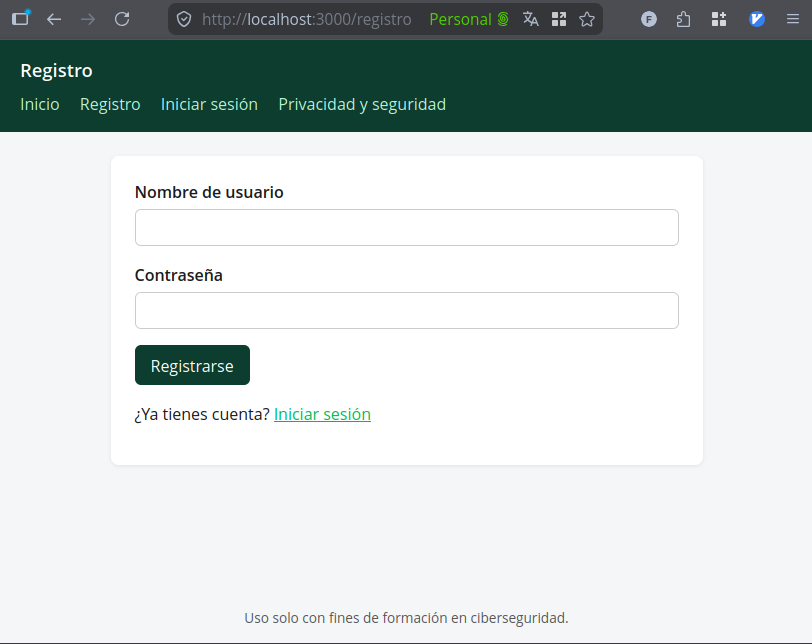
\includegraphics[width=0.9\textwidth,keepaspectratio]{img/1/1.1-registro.png}
    \caption{Interfaz de registro del sitio web de prueba.}
    \label{fig:reg_inicio}
\end{figure}

A continuación, se abrieron las herramientas de desarrollador del navegador para inspeccionar los recursos cargados. En la pestaña de red (\textit{Network}), se localizó el archivo \texttt{crypto-client.js}, el cual es responsable de la lógica criptográfica en el cliente, tal como se observa en la Figura \ref{fig:reg_network}.

\begin{figure}[H]
    \centering
    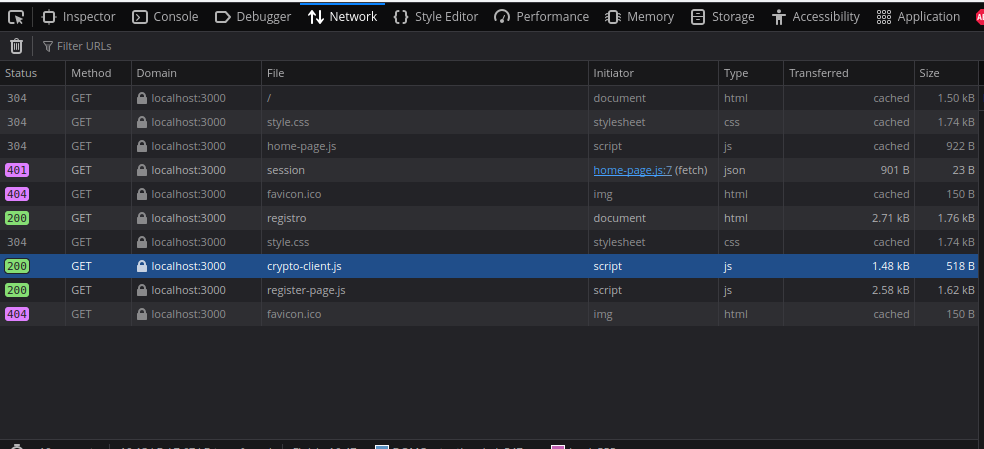
\includegraphics[width=0.9\textwidth,keepaspectratio]{img/1/1.2-networkCryptoClientJs.png}
    \caption{Identificación del archivo \texttt{crypto-client.js} en el tráfico de red.}
    \label{fig:reg_network}
\end{figure}

Al analizar el contenido de dicho archivo, se identificó la función \texttt{hashPasswordUtf8}, la cual utiliza la API \texttt{crypto.subtle.digest} con el algoritmo \textbf{SHA-256}. Esta evidencia se presenta en la Figura \ref{fig:reg_sha}.

\begin{figure}[H]
    \centering
    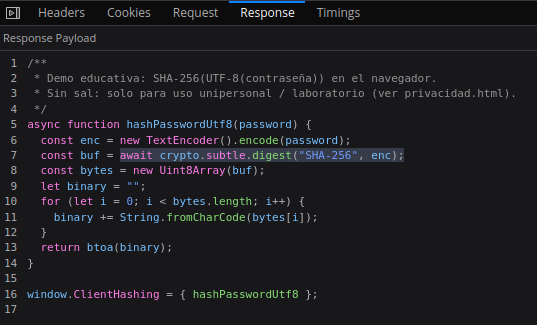
\includegraphics[width=0.9\textwidth,keepaspectratio]{img/1/1.3-responseCryptoClientJs.png}
    \caption{Confirmación del uso de SHA-256 en el código fuente.}
    \label{fig:reg_sha}
\end{figure}

Posteriormente, se verificó cómo se integra esta función en el flujo de registro. En la Figura \ref{fig:reg_page_net} se observa la carga del script \texttt{register-page.js}, que gestiona el formulario de inscripción.

\begin{figure}[H]
    \centering
    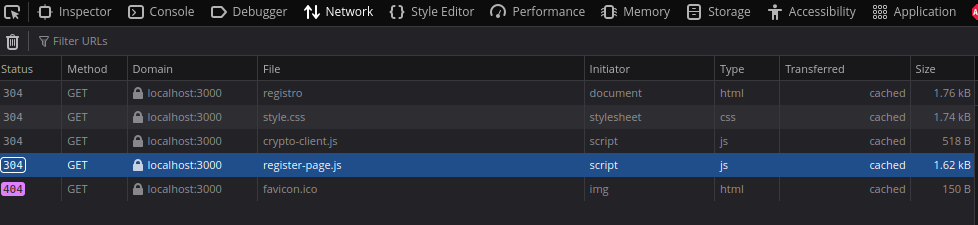
\includegraphics[width=0.9\textwidth,keepaspectratio]{img/1/1.4-networkRegisterPageJs.png}
    \caption{Localización del script \texttt{register-page.js}.}
    \label{fig:reg_page_net}
\end{figure}

Finalmente, al revisar el código de \texttt{register-page.js}, se confirmó que los datos del formulario son procesados por la función de hashing antes de ser enviados al servidor mediante una petición \texttt{fetch}, como se detalla en la Figura \ref{fig:reg_final}.

\begin{figure}[H]
    \centering
    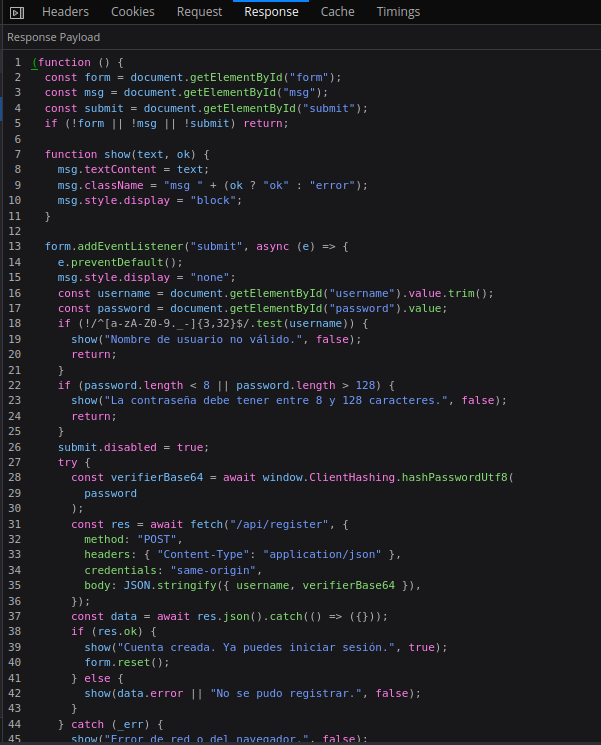
\includegraphics[width=0.9\textwidth,height=0.7\textheight,keepaspectratio]{img/1/1.5-responseRegisterPageJs.png}
    \caption{Llamada a la función de hashing en el proceso de registro.}
    \label{fig:reg_final}
\end{figure}

\clearpage

\subsection{Identifica el algoritmo de hash utilizado al momento de iniciar sesión}
Para el proceso de inicio de sesión, se siguió una metodología similar. Primero se navegó a la interfaz de login, visible en la Figura \ref{fig:log_inicio}.

\begin{figure}[H]
    \centering
    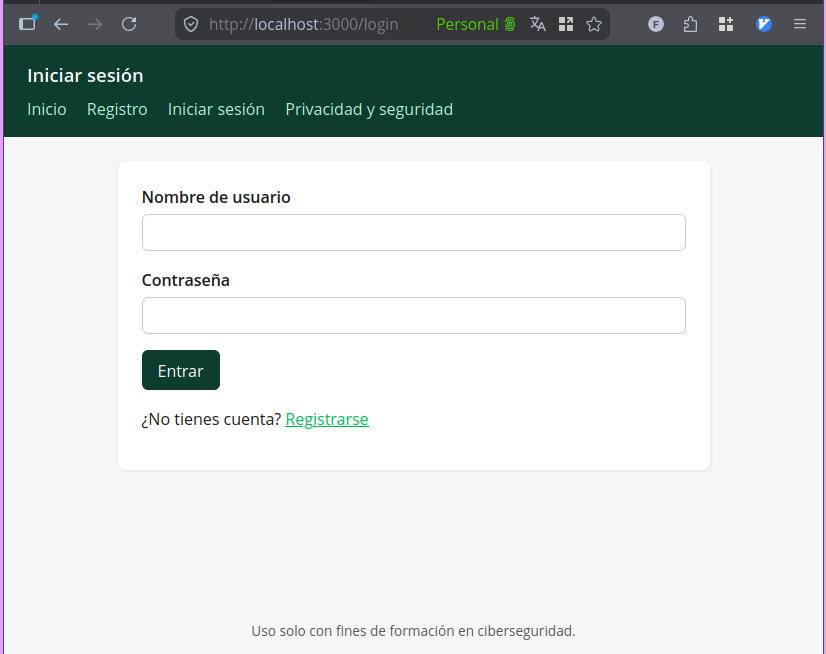
\includegraphics[width=0.9\textwidth,keepaspectratio]{img/2/2.1-login.png}
    \caption{Interfaz de inicio de sesión.}
    \label{fig:log_inicio}
\end{figure}

Se inspeccionó nuevamente el tráfico de red para validar qué scripts controlan este formulario, identificando el archivo \texttt{login-page.js}, como se muestra en la Figura \ref{fig:log_network}.

\begin{figure}[H]
    \centering
    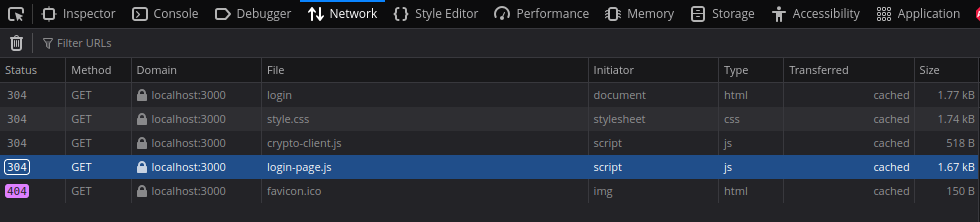
\includegraphics[width=0.9\textwidth,keepaspectratio]{img/2/2.2-networkLoginPageJs.png}
    \caption{Detección del script \texttt{login-page.js}.}
    \label{fig:log_network}
\end{figure}

Al examinar el código de la respuesta, se comprobó que el sitio web reutiliza la misma lógica de \texttt{SHA-256} definida en el cliente para procesar la contraseña del usuario antes de la autenticación. Este paso final de verificación se ilustra en la Figura \ref{fig:log_final}.

\begin{figure}[H]
    \centering
    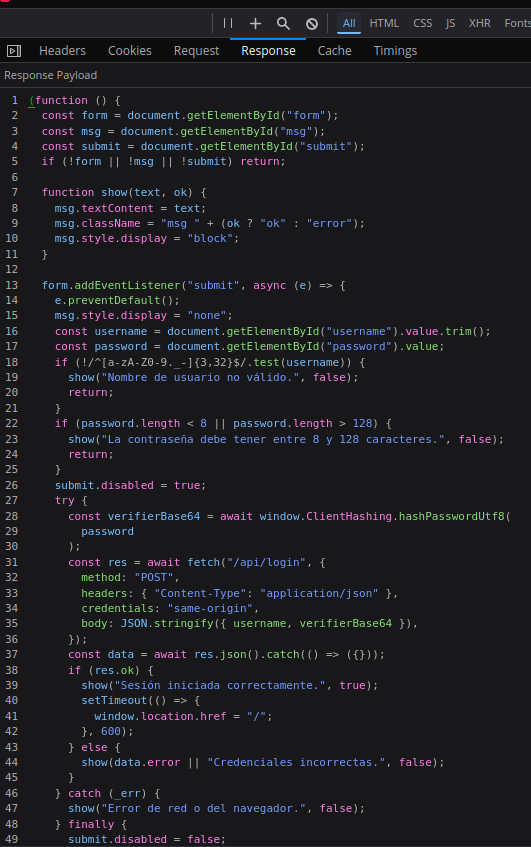
\includegraphics[width=0.9\textwidth,height=0.7\textheight,keepaspectratio]{img/2/2.3-responseLoginPageJs.png}
    \caption{Uso consistente de SHA-256 durante el inicio de sesión.}
    \label{fig:log_final}
\end{figure}

\clearpage

\subsection{Genera el hash de la contraseña desde la consola del navegador}
Para emular el comportamiento de la aplicación y obtener el valor real que se envía al servidor, se replicó la lógica criptográfica utilizando la consola del desarrollador del navegador. El procedimiento consistió en codificar la contraseña en texto plano a UTF-8, aplicar la función de resumen SHA-256 utilizando la API nativa \texttt{crypto.subtle.digest}, y finalmente convertir el buffer de bytes resultante a una cadena en formato Base64. 

El código ejecutado para realizar esta transformación es el siguiente:
\begin{verbatim}
(async () => {
   const p = "pepe1234";
   const enc = new TextEncoder().encode(p);
   const buf = await crypto.subtle.digest("SHA-256", enc);
   const b64 = btoa(String.fromCharCode(...new Uint8Array(buf)));
   console.log("Tu hash en Base64 es:", b64);
})();
\end{verbatim}

La Figura \ref{fig:generacion_hash} demuestra la ejecución exitosa de este script en la consola, retornando el hash en Base64 que representa la contraseña \texttt{"pepe1234"}.

\begin{figure}[H]
    \centering
    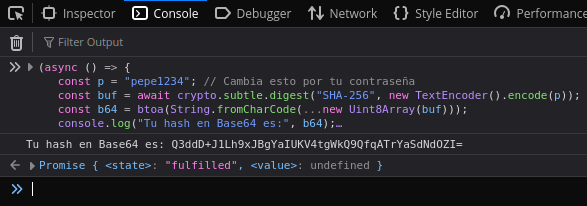
\includegraphics[width=0.95\textwidth,keepaspectratio]{img/3/3.1-obtencionHash.png}
    \caption{Ejecución del script en consola y obtención del hash en Base64.}
    \label{fig:generacion_hash}
\end{figure}

\clearpage

\subsection{Intercepta el tráfico login con BurpSuite}
Para auditar la comunicación entre el cliente y el servidor, se procedió a configurar un proxy de interceptación utilizando la herramienta Burp Suite. El primer paso consistió en asegurar que el interceptor estuviera activo en la pestaña \texttt{Proxy}, como se observa en la Figura \ref{fig:proxy_on}.

\begin{figure}[H]
    \centering
    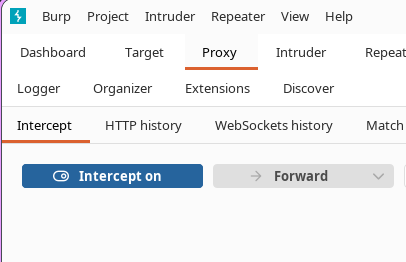
\includegraphics[width=0.7\textwidth,keepaspectratio]{img/4/4.1-inProxyOption.png}
    \caption{Activación del modo Intercept en Burp Suite.}
    \label{fig:proxy_on}
\end{figure}

Posteriormente, se navegó a la página de inicio de sesión de la aplicación. Se utilizó la cuenta creada anteriormente con el nombre de usuario \texttt{"pepe"} (cuya contraseña real es \texttt{"pepe1234"}). Sin embargo, con el objetivo de capturar una petición fallida para su posterior manipulación, se completó el formulario ingresando una clave deliberadamente incorrecta: \texttt{"clavefalsa"}, tal como se muestra en la Figura \ref{fig:login_form}.

\begin{figure}[H]
    \centering
    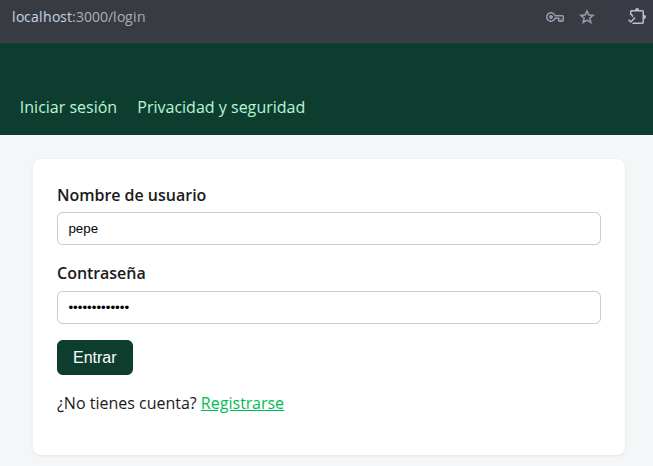
\includegraphics[width=0.8\textwidth,keepaspectratio]{img/4/4.2-loginForm.png}
    \caption{Formulario de inicio de sesión completado con credenciales incorrectas.}
    \label{fig:login_form}
\end{figure}

Al presionar el botón de inicio de sesión, Burp Suite capturó la petición HTTP saliente. En la Figura \ref{fig:request_post} se puede apreciar la captura de la petición \texttt{POST} dirigida al endpoint \texttt{/api/login}, la cual quedó retenida en el proxy a la espera de ser procesada o modificada.

\begin{figure}[H]
    \centering
    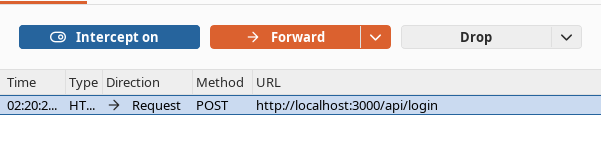
\includegraphics[width=0.8\textwidth,keepaspectratio]{img/4/4.3-requestPost.png}
    \caption{Petición POST interceptada por Burp Suite.}
    \label{fig:request_post}
\end{figure}

\clearpage

\subsection{Realiza el intento de login}
Con la petición interceptada, se inició la fase de explotación del ataque Pass the Hash. Primero, se inspeccionó el cuerpo de la petición original en formato JSON. En la Figura \ref{fig:payload_original} se observa el parámetro \texttt{verifierBase64}, el cual contiene el hash SHA-256 correspondiente a la contraseña incorrecta (\texttt{"clavefalsa"}).

\begin{figure}[H]
    \centering
    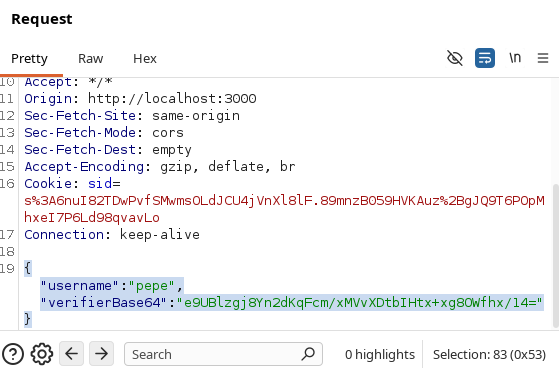
\includegraphics[width=0.95\textwidth,keepaspectratio]{img/4/4.4-payloadOriginal.png}
    \caption{Payload original con el hash de la contraseña incorrecta.}
    \label{fig:payload_original}
\end{figure}

A continuación, se procedió a modificar este parámetro manualmente dentro de Burp Suite. Se reemplazó el valor original por el hash Base64 obtenido previamente en la sección 2.3 del informe (el hash legítimo de \texttt{"pepe1234"}). La Figura \ref{fig:payload_hacked} muestra el payload ya manipulado antes de ser reenviado (\textit{forwarded}) al servidor.

\begin{figure}[H]
    \centering
    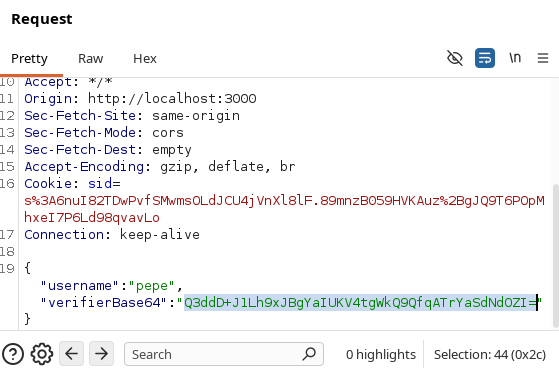
\includegraphics[width=0.95\textwidth,keepaspectratio]{img/4/4.5-payloadHacked.png}
    \caption{Payload manipulado con el hash real inyectado manualmente.}
    \label{fig:payload_hacked}
\end{figure}

Una vez enviada la petición modificada, se regresó al navegador para verificar el resultado. A pesar de haber ingresado \texttt{"clavefalsa"} en el formulario, el servidor validó el hash inyectado y permitió el acceso, como se evidencia en el mensaje de éxito de la Figura \ref{fig:sesion_ok}.

\begin{figure}[H]
    \centering
    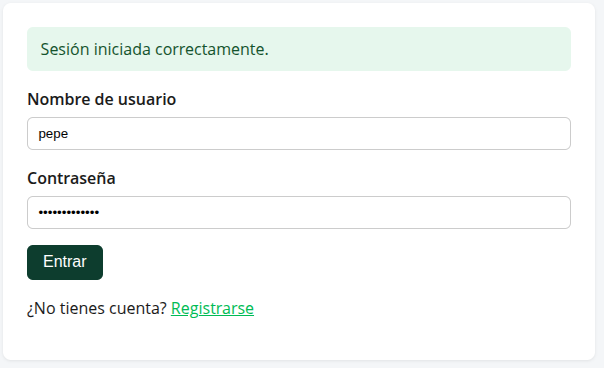
\includegraphics[width=0.8\textwidth,keepaspectratio]{img/4/4.6-sesionIniciada.png}
    \caption{Confirmación de sesión iniciada exitosamente tras el ataque.}
    \label{fig:sesion_ok}
\end{figure}

Finalmente, la Figura \ref{fig:sesion_activa} muestra la página de inicio con la sesión activa del usuario \texttt{"pepe"}, demostrando que el conocimiento del hash es suficiente para suplantar la identidad del usuario sin poseer la contraseña original.

\begin{figure}[H]
    \centering
    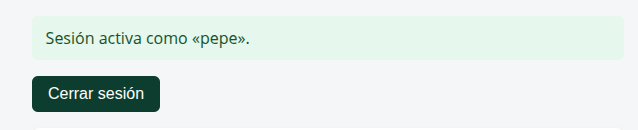
\includegraphics[width=0.8\textwidth,keepaspectratio]{img/4/4.7-sesionActiva.png}
    \caption{Vista de la sesión activa en la página principal.}
    \label{fig:sesion_activa}
\end{figure}

\clearpage

\subsection{Identifica las políticas de privacidad o seguridad}
Al revisar la sección correspondiente del sitio web (disponible en \url{http://localhost:3000/privacidad}), se constata que la plataforma declara explícitamente su mecanismo de manejo de credenciales. La política informa a los usuarios que las contraseñas no se transmiten en texto plano, sino que son procesadas localmente mediante el algoritmo SHA-256 antes de su envío.

Desde la perspectiva de una auditoría de ciberseguridad, destaca la inusual transparencia del documento al admitir las debilidades de su propia arquitectura. La política reconoce explícitamente la ausencia de "sal" (salt) criptográfica y advierte que la interceptación del resumen permitiría su reutilización, validando teóricamente la viabilidad del ataque \textit{Pass the Hash} ejecutado en la sección anterior. Asimismo, detalla que el servidor únicamente conserva el nombre de usuario, el verificador SHA-256 y una cookie de sesión \texttt{HttpOnly}. Aunque la declaración cumple con el principio de transparencia informativa, a nivel técnico confirma un diseño inherentemente inseguro para entornos de producción, ya que transforma el hash interceptable en el equivalente a una contraseña en texto plano.

\subsection{Demuestra 4 conclusiones sobre la seguridad}

Tras la auditoría realizada, se presentan las siguientes conclusiones técnicas:

\begin{enumerate}
    \item \textbf{Vulnerabilidad del hash como equivalente a texto plano:} El laboratorio demostró que, al hashear la contraseña solo en el cliente, el hash resultante se convierte en el nuevo secreto de autenticación. Como el servidor no pide la contraseña original sino este código, cualquier atacante que intercepte el hash puede entrar a la cuenta sin conocer jamás la clave real del usuario.
    
    \item \textbf{Efectividad del ataque Pass the Hash (PtH):} La manipulación exitosa de la petición con Burp Suite confirmó que el sistema es vulnerable a ataques de reuso de credenciales. Al inyectar un hash válido en una petición fallida, se comprobó que el servidor no tiene mecanismos para distinguir entre un cálculo legítimo del navegador y una inyección manual de un tercero.
    
    \item \textbf{Riesgo por falta de sal (Salt):} La ausencia de sal criptográfica personalizada por usuario facilita ataques de diccionario o tablas precomputadas. Si dos usuarios eligen la misma contraseña, sus hashes en la base de datos serán idénticos, lo que permite a un atacante comprometer múltiples cuentas simultáneamente una vez que descifra un solo valor.
    
    \item \textbf{Inseguridad del hashing de un solo paso:} El uso de un único SHA-256 es insuficiente para proteger credenciales modernas. Una implementación segura debería realizar el hashing principalmente en el servidor utilizando funciones lentas y costosas (como Argon2 o bcrypt) diseñadas para resistir ataques de fuerza bruta, en lugar de confiar únicamente en un resumen rápido ejecutado en el navegador.
\end{enumerate}

\end{document}
